% ACM
%\documentclass[sigconf]{acmart}

% Manuscript
\documentclass[10pt,twocolumn]{article}
\usepackage[numbers]{natbib}

\usepackage{booktabs} % For formal tables

% Document-specific packages
\usepackage{epigraph}
\usepackage[normal]{threeparttable}
\usepackage{graphicx}

% Document-specific definitions
\newcommand{\beq}{\begin{eqnarray}}
\newcommand{\eeq}{\end{eqnarray}}
\newcommand{\+}{\phantom{-}}

% Copyright
%\setcopyright{none}
%\setcopyright{acmcopyright}
%\setcopyright{acmlicensed}
%\setcopyright{rightsretained}
%\setcopyright{usgov}
%\setcopyright{usgovmixed}
%\setcopyright{cagov}
%\setcopyright{cagovmixed}


% DOI
%\acmDOI{10.475/123_4}

% ISBN
%\acmISBN{123-4567-24-567/08/06}

%Conference
%\acmConference[WOODSTOCK'97]{ACM Woodstock conference}{July 1997}{El
%  Paso, Texas USA} 
%\acmYear{1997}
%\copyrightyear{2016}

%\acmPrice{15.00}

\begin{document}
\title{Network Structure, Efficiency, and Performance in WikiProjects}

% ACM
%\author{Edward L. Platt}
%\affiliation{%
%  \institution{University of Michigan}
%  \city{Ann Arbor} 
%  \state{Michigan} 
%}
%\email{elplatt@umich.edu}

% Manuscript
\author{Edward L. Platt \\ University of Michigan \\ Ann Arbor, Michigan \\ elplatt@umich.edu}

% The default list of authors is too long for headers}
%\renewcommand{\shortauthors}{B. Trovato et al.}


% ACM
% The code below should be generated by the tool at
% http://dl.acm.org/ccs.cfm
% Please copy and paste the code instead of the example below. 
%
%\begin{CCSXML}
%\end{CCSXML}

% ACM
%\ccsdesc[500]{Computer systems organization~Embedded systems}
%\ccsdesc[300]{Computer systems organization~Redundancy}
%\ccsdesc{Computer systems organization~Robotics}
%\ccsdesc[100]{Networks~Network reliability}


% ACM
% \keywords{collaboration, peer production, wikipedia}

\maketitle

\begin{abstract}
The internet has enabled collaborations at a scale never before possible,
but the best practices for organizing such large collaborations are still not clear.
Wikipedia is a visible and successful example of such a collaboration which might offer
insight into what makes large-scale, decentralized collaborations successful.
We analyze the relationship between the structural properties of WikiProject coeditor networks
and the performance and efficiency of those networks.
We also perform numerical simulations to determine whether social learning on an NK model can
reproduce the behavior observed on Wikipedia.
We find several results seen in numerical and small-scale lab studies:
a trade-off between performance and efficiency and
higher performance with less skewed node distributions and shorter path lengths.
We also see behaviors not previously identified: an association between low degree coeditor networks
and both higher performance and higher efficiency,
suggesting possible benefits to decentralized collaborations made of smaller, more tightly-knit teams.
We also propose a novel consensus-based social learning strategy that is both more efficient and higher
performance than existing strategies, and reproduces some behaviors seen in WikiProjects.
\end{abstract}

\section{Introduction}
\epigraph
{The problem with Wikipedia is that it only works in practice. In theory, it's a total disaster.}
{Gareth Owen \cite{elsharbaty_editing_2016} }

The internet has enabled collaborations at a scale never before possible, a global scale.
Wikipedia is one of the most successful and visible of these collaborations,
and is particularly interesting for its highly decentralized structure with very little top-down control.
It is notoriously difficult to organize even small groups without top-down control,
and yet Wikipedia, with millions of editors, somehow functions.
A better theoretical understanding of projects like Wikipedia is highly desirable as it could
help inform the design of new collaborative projects.
We focus on one aspect of organizing a large-scale decentralized collaboration: the network structure.
If Wikipedia is not structured as a top-down hierarchy, how is it structured?
And how does that structure influence its success?

We approach these questions by analyzing WikiProjects on the English-language Wikipedia.
WikiProjects are collections of thematically related articles,
each with their own standards, norms, and processes for evaluating and improving articles.
We analyze the coeditor networks of these projects: which editors have worked together on at least
one article?
In particular, we examine the relationship between the structure of a project's coeditor network
and the performance and efficiency of its articles.
Performance represents the ability of a project to get articles to a high quality level,
while efficiency represents the ability to improve articles of any level quickly.
We also perform numerical simulations to compare the behavior observed on Wikipedia to the results
of several variants of a simple networked social learning model.

Our main findings are:
\begin{itemize}
\item WikiProjects having low-degree coeditor networks tend to have both higher performance and higher efficiency, independent of path lengths;
\item Short path lengths tend to be associated with higher performance, consistent with a conformity-based learning strategy;
\item Structural inequality, as measured by degree skewness, is associated with lower performance,
and lower efficiency at reaching the highest quality levels;
\item Using numerical simulations, we show that the performance and efficiency of some networked learning strategies depends on degree.
\end{itemize}

The rest of the paper is structured as follows.
Section \ref{sec:background} reviews related work and the motivation for the present project,
Section \ref{sec:wp} describes the methodology and results of our empirical analysis of WikiProjects,
Section \ref{sec:sim} describes the methodology and results of our numerical simulations,
Section \ref{sec:discuss} discusses the interpretation and broader impact of our results,
and Section \ref{sec:conclusion} concludes.

\section{Background and Related Work}
\label{sec:background}

In the field of social learning,
much research has been done to understand how groups of agents
can solve problems collaboratively.
In {\em networked social learning}, agents are represented by nodes on a network
and can only interact with their neighbors.
Social learning tasks can be divided into cases where agents have {\em generated signals}
(independently noisy estimates of a true value)
and those where agents have {\em interpreted signals}
(solutions based on different internal models of available data)
\cite{hong_interpreted_2009}.
For generated signals,
a naive Bayesian approach converges to the truth when conditions
on the network's degree distribution,
while the speed of convergence depends on the {\em spectral gap}
between the two largest eigenvalues of the network's adjacency matrix
\cite{golub_naive_2010}.
Complex social learning tasks can also be modeled as the problem
of maximizing an objective function with many local maxima,
referred to as a {\em rugged landscape}
\cite{lazer_network_2007, mason_propagation_2008, mason_collaborative_2012, grim_scientific_2013, barkoczi_social_2016}.
Numerical simulations have shown that efficient networks (those with short paths between nodes)
can allow less exploration of possible solutions,
resulting in a fast convergence to a non-optimal solution \cite{mason_propagation_2008, grim_scientific_2013}.
However, when conformity-based social learning strategies are used, efficient networks can outperform
inefficient ones \cite{barkoczi_social_2016}.

Lab-based experiments on networked collaboration
suggest a complex interaction between network topology,
and other factors.
While groups of networked human subjects reliably perform very well on
difficult graph-coloring tasks, the best performing network architectures
(e.g., fully-connected vs. small-world) vary
from task to task \cite{kearns_experiments_2012}.
The same studies found that while human subjects tend to perform very well on
a number of networks, they perform worst on collaboratively self-organized
networks, highlighting the importance of intentionality
in constructing communication channels for collective decision-making.
Similarly, some network topologies are able to reach faster decisions in the
presence of more information, while others show the opposite effect
\cite{kearns_experimental_2006}.
Based on lab experiments, Fowler and Christakis \cite{fowler_cooperative_2010}
suggest that individual decisions towards altruism are conditional on their
neighbor's behavior and ``contagious'' up to three degrees away.
Later experiments by Suri and Watts \cite{suri_cooperation_2011} confirmed the
existence of conditional altruism,
but concluded that altruistic
behavior only influences first-degree neighbors.
While theories of networked social learning have been tested in small-scale lab experiments,
there is a need to study real-world, large-scale collaborations,
as we do in the present paper.

In addition to learning, decision-making is a crucial component of collaboration.
The Condorcet jury theorem and its extensions \cite{list_epistemic_2001}
describe how individuals can use majority voting to improve their
decision-making ability.
The process of decision-making is sometimes divided into
``talking'' and ``voting'' stages.
While hierarchical representative democracy sometimes improves the outcome
of ``talk,'' it weakens the result of the Condoret jury theorem for voting
\cite{list_epistemic_2001}.
Robert Michels proposed the ``iron law of oligarchy,''
\cite{michels_political_1999} which states that
the earlier members of a group will, over time, gain disproportionate
decision-making power and act increasingly out of self-interest rather than
the good of the group.
Shaw and Hill found that behavior in online wiki communities is consistent
with the iron law \cite{shaw_laboratories_2014}.
A number of studies, summarized in \cite{gentry_consensus_1982},
have examined consensus-based decision-making procedures, used extensively by
the Quakers and later by activist communities.
The hallmark of consensus is the equal and active participation by all members
of a group.
Key findings include the trade-off between speed and quality of decisions,
the importance of expressing conflict early in the process,
and the willingness to recognize when one's own views are counter to the
existing consensus.
De Tar created InterTwinkles \cite{detar_intertwinkles:_2013},
an online suite of tools to facilitate consensus decision-making
in small cooperatives.
Consensus decision making is notoriously difficult to apply in large groups.
Wikipedia is one of the largest collaborations to use consensus-based
decision-making,
making it an excellent place to study the role of network structure in
large-scale collaboration.

Research on digital communities has also examined some non-network factors
influencing the quality of decisions and collaborative work.
Using a simulation model, Hong and Page \cite{hong_groups_2004} found that
diverse groups can outperform groups composed of the best individual
problem-solvers.
In sociology, much research has been done examining the relationship between
network structure and social capital.
Powerful individuals are often ``brokers''
who act as exclusive intermediaries between disconnected portions of the
social network \mbox{\cite{silverman_patronage_1965}}.
Similarly, successful innovation in organizations often occurs in ``structural
holes'' between groups \mbox{\cite{granovetter_strength_1973}}.
There is some evidence that groups with high structural inequality,
as evidenced by highly-skewed degree distributions,
perform worse on collaborative tasks \mbox{\cite{kearns_experiments_2012}}.
In the present project, we examine the effect of structural inequality
on collaboration in Wikipedia.

Several studies have examined the role of community in the specific context
of Wikipedia.
Robert and Romero found that
larger group sizes yield higher article ratings
(as determined by editor peer-review)
when the groups are diverse and experienced
\cite{robert_when_2015}.
Also on Wikipedia,
Kittur and Kraut found that different types of coordination have a complex
effect on the quality of Wikipedia articles \cite{kittur_harnessing_2008}.
Both explicit and implicit coordination result in higher quality articles,
with explicit coordination being especially central in the early life of an
article.

Across the broad range of work on collaboration and related topics,
a few key themes emerge.
The efficiency and performance of collaborations are important considerations
and vary depending on both network structure and type of task.
While social learning predicts no relationship between the two,
contagion-style innovation models predict a trade-off.
Such a trade-off has been observed in simulations and lab experiments on
collaboration.
In this project, I will investigate several gaps in the existing literature.
In much of the existing literature,
degree distribution correlate to performance.
But aside from the naive Bayes case in social learning, it is unknown whether
the correlation is explained best by degree or by another structural property
correlated with degree.
The characteristic path length and min-cut studied here are candidates for such
degree-correlated factors.
While existing work has focused on families of artificial networks,
this project examines a large number of naturally-occurring networks.
Unlike artificial networks, the structural properties of these naturally-occurring
networks can vary independently, making it easier to isolate individual
network properties that correlate with outcome variables.
This project will also examine Wikipedia for evidence that structural
inequality (in the form of skewed
degree distributions) has a detrimental effect on performance,
as has been observed in lab experiments
\mbox{\cite{kearns_experiments_2012}}.

\section{WikiProjects}
\label{sec:wp}

\subsection{Data}

Our analysis combines multiple data sets from the English-language Wikipedia.
For information about edit history, we used a publicly-available data set containing
metadata about all edits from July 12, 2006 to December 2, 2015.
To get the rating history of each article,
we wrote a script to scrape the daily logs produced by WP 1.0 Bot for each WikiProject
between May 4, 2006 and December 2, 2015.
Finally, we used a publicly-available log of page events (including rename events)
to reconstruct the unique identifier for each article title mentioned in the rating history logs.

\subsection{Efficiency and Performance}

To model the relationship between performance, efficiency, and network structure,
we must have a way to quantify performance and efficiency.
We define these quantities on a per-WikiProject basis to enable comparisons across different
projects.
Our definitions are inspired by work modeling collective problem-solving as an optimization
problem \cite{lazer_network_2007, mason_propagation_2008, mason_collaborative_2012,
grim_scientific_2013, barkoczi_social_2016}.
The efficiency quantifies how quickly a solution is reached,
while the performance quantifies how good the eventual solution is.

For a WikiProject, efficiency quantifies how quickly project participants can improve the
assessed quality of an article.
Quality assessments are made through consensus of the project participants themselves,
so different projects can have different standards and practices for assessing article quality.
So the efficiency is not a measure of how quickly some objective measure of quality improves,
but rather of how quickly the project participants can reach consensus on the improvements that
need to be made and make those improvements.
Because our definition relies on assessment transitions, we define efficiency variables for
each of the project-level quality assessments: A, B, and C.
If $T(W,G)$ is the set of transitions in project $W$ from below grade $G$ to grade $G$ (or higher),
then we quantify the efficiency $E(W,G)$ as:
\beq
E(W,G) &=& \frac{1}{|W(P,G)|} \sum_{t \in W(P,G)} \left[ \frac{r(t)}{g(t)} \right]^{-1},
\eeq
where $r(t)$ is the number of revisions since the previous grade transition,
and $g(t)$ is the number of grade levels crossed by transition $t$.
The $g(t)$ term is added because an assessments often raise article quality by several
grades, in which case the revisions are divided evenly between all grade levels achieved.
It is also worth noting that we measure efficiency in terms of revisions made,
rather than time passed.
We focus on revisions because the amount of work done on an article varies widely from day to day.

For performance, we wish to quantify how good articles tend to be when they reach a stable state.
Measuring performance is difficult for several reasons:
there is no objective measure of article quality available,
and articles are always changing, making it difficult to know which articles should be considered
complete or stable.
We use an extremely simple performance measure that gives surprisingly consistent results.
In addition to per-project quality assessment, articles can be given ``featured article'' or
``good article'' status.
The criteria for these statuses are consistent across all of Wikipedia,
and any editor can participate in the discussion and decision to award good or featured
status.
In other words, the good and featured statuses are more objective than per-project assessments.
Our performance measure $P(W)$ is just the percentage of articles in project $W$ which have reached
good or featured status:
\beq
P(W) &=& \frac{f(W) + g(W)}{n(W)},
\eeq
where $f(W)$ and $g(W)$ are the numbered of featured and good articles respectively,
and $n(W)$ is the total number of articles.

\subsection{Coeditor Networks}

For each WikiProject, we compare the efficiency and performance measures to the structural
properties of its coeditor network.
The {\em coeditor network} of a WikiProject consists of nodes representing editors.
Two editors are connected when they have both edited the same article or talk page.
The edges are directed, with the direction representing the direction of
{\em plausible information flow};
an edge from editor A to editor B exists if A edited an article and then B edited the same article at
a later time.
Edges can exist in both directions e.g., if an article was edited first by A, then by B, and again by A.
For simplicity, we assign all edges unit weight.
We focus on three structural properties: degree, characteristic path length, and min-cut.

The node degree distribution is the simplest structural property we analyze for WikiProject
coeditor networks.
The in-degree (out-degree) of a node is the number of edges to (from) that node.
Taking the average of either in-degree or out-degree gives the same value:
the {\em mean degree} of the network.
In our context, the mean degree represents how many others a given editor has collaborated with.
We also consider the {\em skewness} of the in-degree and out-degree distributions.
A large positive degree skewness value for a WikiProject coeditor network
implies that a small number of editors have a very large number of collaborators,
while a small positive value implies that the editors having the most collaborators
don't have many more than a typical editor.

We also calculate the characteristic path length for each WikiProject coeditor network.
The {\em distance} from editor A to editor B is the length of the shortest path from A to B.
The {\em characteristic path length} is the mean distance between all editor pairs.
If no path exists between two editors, we exclude that pair from the mean.
For brevity, we will simply refer to this quantity as the {\em path length}.
The path length represents how quickly information can move through the network.
Networks with longer paths require more interactions for information to propagate through
the network,
which has been shown to reduce efficiency in some settings
\cite{mason_propagation_2008,barkoczi_social_2016}.

Our final network measure quantifies the connectivity of a project's coeditor network using
min-cut size.
The minimum $st$-cut between nodes $s$ and $t$ is the set of edges that must be removed in order that
no path exists from $s$ to $t$.
The minimum cut (min-cut) of a graph is the smallest minimum $st$-cut over all node pairs $st$. 
The size of the graph min-cut quantifies the connectivity of a graph,
but only incorporates information about edges lying on paths crossing the min-cut.
Instead, we use the mean size of all minimum $st$-cuts, which we refer to as the
{\em mean min-cut}.
This measure quantifies the number of redundant paths information can take through the network.
Networks with higher redundancy are more resilient to errors on one path \cite{albert_error_2000}
and allow innovations to propagate through complex contagion,
in which innovations are only adopted after multiple exposures through different sources
\cite{centola_complex_2007}.

The mean path and min-cut network measures are computationally intensive,
requiring distance and minimum $st$-cut calculations for each all node pairs.
For larger projects, these calculations are impractical.
When coeditor networks were large, we employed sampling to determine mean path length and mean
min-cut.
For mean path length, source nodes were sampled, and path length was calculated to all destination nodes
from each of these.
For min-cut, node pairs were sampled.
In both cases, stratification was used to ensure the same number of nodes were were sampled from each of
12 node degree quantiles.
We estimated the error due to sampling by determining true values for a medium-sized project,
and calculating error as a function of sample-size.
Sample sizes were chosen such that relative error was below 10\%.
Even with sampling, however, it was impractical to calculate these properties for the largest projects,
so we exclude them from the analysis.
To control for bias in project size, we include several size-related variables in our models.

\subsection{Regression Models}

\begin{table*}[!ht]
\small
\caption{Standardized coefficients for OLS models.
\label{tab:model}
}
\bigskip
\begin{tabular}{lllllllll}
\hline
                               & Perf$^\dagger$ & Perf$^\dagger$ & A-Eff$^\dagger$ & A-Eff$^\dagger$ & B-Eff$^\dagger$ & B-Eff$^\dagger$ & C-Eff$^\dagger$ & C-Eff$^\dagger$ \\
\hline
Mean degree$^\dagger$          &  -0.84$^{***}$  &  -0.78$^{***}$
                               &  -0.61$^{**}$   &  -0.84$^{***}$
                               &  -0.50$^{***}$  &  -0.61$^{***}$
                               &  -0.34$^{**}$   &  -0.31$^{*}$ \\
In-degree skewness$^\dagger$   &  -0.58$^{***}$  & \+ ---      
                               &  -0.43$^{**}$   & \+ ---      
                               &  -0.19          & \+ ---      
                               &  -0.1           & \+ ---      \\
Out-degree skewness$^\dagger$  &  \+ ---         &  -0.48$^{***}$  
                               &  \+ ---         &  -0.57$^{***}$
                               &  \+ ---         &  -0.26$^{*}$
                               &  \+ ---         &  -0.066 \\
Mean path$^\dagger$            &  -0.357$^{***}$ &  -0.356$^{***}$ 
                               &  -0.026         &  -0.096
                               &  -0.020         &  -0.045
                               &  -0.092$^{**}$  &  -0.086 \\
C-eff$^\dagger$                &  -0.083$^{**}$  & -0.085$^{**}$  
                               &  \+ ---         & \+ ---      
                               &  \+ ---         & \+ ---      
                               &  \+ ---         & \+ --- \\
Connectivity                   & \+0.018         & \+0.016        
                               & \+0.081         & \+0.088
                               & \+0.126$^{***}$ & \+0.142$^{***}$
                               & \+0.080$^{**}$  & \+0.081$^{**}$ \\
Mean editors/article$^\dagger$ & \+0.37$^{***}$  & \+0.40$^{***}$ 
                               & \+0.22          & \+0.27
                               & \+0.20          & \+0.22$^{*}$
                               & \+0.076         & \+0.075 \\
Article count$^\dagger$        &  -0.32          & -0.27          
                               & \+0.63${^*}$    & \+0.70${^*}$ 
                               & \+0.76$^{**}$   & \+0.78$^{**}$
                               & \+0.67$^{***}$  & \+0.67$^{***}$ \\
Editor count$^\dagger$         & \+0.68$^{*}$    & \+0.48         
                               & \+0.74$^{*}$    & \+0.97$^{**}$
                               & \+0.60$^{*}$    & \+0.72$^{**}$
                               & \+0.52$^{*}$    & \+0.46$^{*}$ \\
Revision count$^\dagger$       & \+0.37          & \+0.39         
                               &  -0.84$^{**}$   & -0.88$^{**}$
                               &  -1.05$^{***}$  & -1.05$^{***}$
                               &  -1.00$^{***}$  & -1.00$^{***}$ \\
First assessment               & \+0.028         & \+0.058        
                               & \+0.086$^{*}$   & \+0.101$^{**}$
                               & \+0.309$^{***}$ & \+0.321$^{***}$
                               & \+0.456$^{***}$ & \+0.460$^{***}$ \\
Mean article age               &  -0.040         & -0.029         
                               &  -0.049         & -0.037
                               &  -0.019         & -0.014
                               &  -0.046$^{*}$   & -0.045$^{*}$ \\
\hline
DoF                            & 1278            & 1278          
                               & 1048            & 1048
                               & 1371            & 1371
                               & 1540            & 1540 \\
R$^2_{adj}$                    & 0.37            & 0.37          
                               & 0.15            & 0.16
                               & 0.30            & 0.30
                               & 0.43            & 0.43 \\
\hline
\end{tabular}
\begin{tablenotes}
\item $\dagger$ Log-transformed. * $p < 0.05$. ** $p < 0.01$. *** $p < 0.001$.
\end{tablenotes}
\end{table*}

We model performance and efficiency in WikiProjects using ordinary least-squares linear regression.
Each WikiProject is taken as a single observation.
The models include each project's coeditor network properties as independent variables.
We also include several project-level variables to control for confounding factors.
The C-efficiency is included in the model for performance to control for the presence of articles
that are actively being improved.
Projects with lower efficiency will have more works-in-progress and could have an artificially low
performance without controlling for efficiency.
Some variables are log-transformed to reduce heteroscedasticity.

Our models are summarized in Table \ref{tab:model}.
Mean min-cut was found to be highly correlated with degree ($r=0.980$, $p<0.001$),
so we exclude min-cut to prevent collinearity.
The high correlation between mean degree and min-cut implies that in most cases
the minimum $st$-cut is simply the either set of edges from $s$ or the set of edges to $t$.
The rarity of non-trivial min-cuts suggests that WikiProject coeditor networks have very few central
bottlenecks and are thus highly decentralized.
In-degree and out-degree skewness were also highly correlated, so each dependent variable was modeled twice:
once with in-degree skewness and once with out-degree skewness.

The regression results are consistent whether in-degree or out-degree skewness is used,
although the out-degree models are slightly more significant when modeling efficiency.
We also see that B-efficiency and C-efficiency have very similar models, but that A-efficiency behaves
differently in its dependence on degree skewness and connectivity.
The different behavior of A-efficiency is likely explained by the observation that the A-Class quality is
infrequently used in practice, meaning that the quality level is usually achieved when an article is rated
as a good or featured article, which involves a different consensus process than lower ratings.

The negative dependence of performance on C-efficiency suggests there is generally a trade-off between
performance and efficiency.
However, low degree is correlated with both higher efficiency and higher performance,
suggesting that it is sometimes possible to improve both simultaneously.
Much of the existing numerical work on networked social learning focuses on path length rather than degree,
so we explore this result further using simulations in the next section.

For path length, we find that longer lengths correspond to lower performance, contrary to the conjecture
that longer path lengths allow more exploration \cite{mason_propagation_2008}
but consistent with a conformity-based social learning strategy \cite{barkoczi_social_2016}.

We also observe that high degree skewness is correlated with lower performance and lower A-efficiency,
suggesting that articles in projects with decentralized coeditor networks reach featured or good status
more efficiently, and reach higher quality ratings in general.

\section{Numerical Simulations}
\label{sec:sim}

We use numerical simulations to determine whether simple models can reproduce the behavior we
observe in WikiProject coeditor networks.
Following existing numerical work on networked social learning
\cite{lazer_network_2007, mason_propagation_2008, mason_collaborative_2012, barkoczi_social_2016},
we use the NK model \cite{kauffman_towards_1987} to create NP-hard, nonlinear optimization problems
and evaluate the effects of network structure and learning strategy on a group's ability to
find solution to those problems.
We are particularly interested in the effect of degree on the efficiency and performance of a group
of networked problem-solving agents.

In the NK model, N loci each have a binary state and value determined by a random lookup table mapping its state
and the state of another K loci to a real number in $[0,1]$.
We report results for the case $N=250$, $K=7$.
Solutions thus take the form of an N-bit string, and the value of the solution is the mean over all loci values.

For a particular problem-solving trial, agents each store their current favored solution and
apply learning strategies to iteratively improve those solutions. We define their
efficiency and performance in terms of the mean solution values for each time step.
We define the performance to be the mean solution value after the process has converged,
while the efficiency is the reciprocal of the number of steps required to converge.
We measure the time to convergence as the number of steps required to reach 99\% of the maximum
mean solution value.

\subsection{Learning Strategies}

Agents can engage in individual learning by applying a hill-climbing algorithm to their current solution.
In each iteration, one bit of the NK solution string is flipped to maximize the solution value.
If no change improves the value, the original solution is kept.
Agents can also incorporate information from any other agents they are connected to by a network edge.
While individual learning always converges to the local maximum relative to the starting point,
social learning strategies allow agents to ``jump'' to drastically different solutions with higher local maxima.

We use both the conformity and best-neighbor strategy from \cite{barkoczi_social_2016}.
In the {\em best-neighbor} strategy, each agent compares its solution to the those of all its
neighbors, and chooses the solution with the highest value.
In the {\em conformity} strategy, agents simply choose the most common solution among their neighbors
(ties are broken uniformly at random).
In both cases, a single iteration of individual learning is performed after each social learning
iteration.

We introduce a new strategy, which we call the consensus strategy.
In {\em consensus}, agents first apply individual learning.
Next, a consensus solution is constructed from each agent's individual solution by setting
each NK locus's state to its most common value among the agent's individual solutions.
The result of this process is that agents accept a single consensus solution at each iteration,
which forms the basis for future individual learning.
We include this strategy because of its similarity to the editing process of Wikipedia:
at any given time, a Wikipedia article has a single state, determined by consensus,
but editors may have differing opinions on how to improve that article.

We also introduce local variants of the above strategies.
The local variants are meant to reflect a more realistic collaboration setting where
individual agents focus on sub-problems.
In these variants, individual learning takes place on a subset of NK loci.
Each agent is associated with an NK locus and the loci its value depends on.
These loci are the agent's {\em concern},
and are the only ones used for individual learning.
Similarly, in the consensus strategy, an NK locus's value is determined only by the agents
concerned with that locus, rather than all agents.

\subsection{Network family}

The agent networks used in our simulations vary from those in previous work in two important ways:
they reflect the structure of the NK model being optimized,
and they allow the degree to be tuned with minimal change to the mean path length.

Our networks are generated by first creating an agent node for each NK locus.
Each node is assigned a concern consisting of its associated locus and all loci its value depends on,
as in the local learning strategies.
This procedure forms an agent-locus affiliation network.
Next, an agent-agent co-affiliation network is created by connecting two agents if they share at least
one locus in their concerns.
This process is exactly analogous to our definition of a WikiProject coeditor network,
with agents playing the role of editors and NK loci playing the role of Wikipedia articles.

To create a tunable degree, we duplicate each node and its node-locus edges and then
randomly rewire those edges before creating the agent-agent network.
The duplication process creates a high overlap between agent concerns,
meaning that most agent-locus edges are redundant and do not create additional agent-agent edges,
resulting in a low average degree.
By randomly rewiring the agent-locus edges, the redundancy is reduced and the average degree of
the agent-agent network is increased.

\subsection{Simulation results}

We simulated 100 trials for rewiring values of 0.0, 0.167, 0.333, 0.5, 0.667, 0.833, and 1.0.
For each trial we generated an NK model with N=250 and K=7 and ran each social learning strategy
for 300 iterations,
as well as a network based on that NK model and rewired.
We confirmed that all trials converged to their maximum value before reaching the last iteration.
Some statistics on the network properties of the networks are summarized in Table \ref{tab:stats}.
We see that the coefficient of variation of degree is approximately 10\%,
while only 1\% for mean path length, confirming that the rewiring process has a stronger influence
on degree than on path length.

\begin{table}
\small
\centering
\caption{
Simulated network statistics.
\label{tab:stats}
}
\bigskip
\begin{tabular}{lcc}
\hline
Property          & Mean  & Std. Dev. \\
\hline
Mean Degree       & 132.3 & 9.2 \\
Mean Path length  & 1.735 & 0.019 \\
\hline
\end{tabular}
\end{table}

\begin{figure}
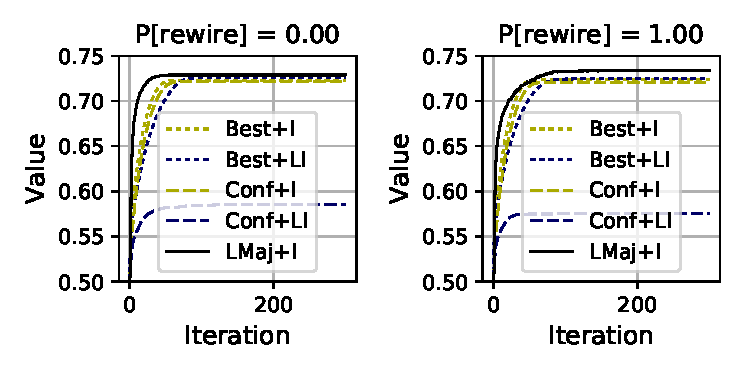
\includegraphics[width=3.33in,height=1.67in]{fig-val-iter.pdf}
\caption{
Mean agent solution value over time, averaged over 100 trials.
The left and right figures show results for agent networks with the probability of
rewiring set to 0 and 1, respectively.
In both, local strategies are less efficient and more performant than non-local.
The consensus strategy is both more efficient and more performant than others,
with its performance increasing with higher rewiring.
\label{fig:val-iter}
}
\end{figure}

\begin{table}
\small
\caption{
Efficiency regression coefficients.
\label{tab:sim-eff}
}
\centering
\bigskip
\begin{tabular}{llc}
\hline
Strategy & Std. Coeff. \\
\hline
Best-neighbor       & -0.064 \\
Conformity          & -0.080 \\
Local best-neighbor & -0.086 \\
Local conformity    & \+0.049 \\
Consensus           & -0.0325$^{***}$ \\
\hline
\end{tabular}
\begin{tablenotes}
\item \centering * $p < 0.05$. ** $p < 0.01$. *** $p < 0.001$.
\end{tablenotes}
\end{table}

\begin{table}
\small
\caption{
Performance regression coefficients.
\label{tab:sim-perf}
}
\centering
\bigskip
\begin{tabular}{llc}
\hline
Strategy & Std. Coeff. \\
\hline
Best-neighbor       & \+0.084 \\
Conformity          & \+0.130 \\
Local best-neighbor & -0.080 \\
Local conformity    & -0.020 \\
Consensus           & \+2.38$\times{10^{-4\;**}}$ \\
\hline
\end{tabular}
\begin{tablenotes}
\item \centering * $p < 0.05$. ** $p < 0.01$. *** $p < 0.001$.
\end{tablenotes}
\end{table}

\begin{figure*}
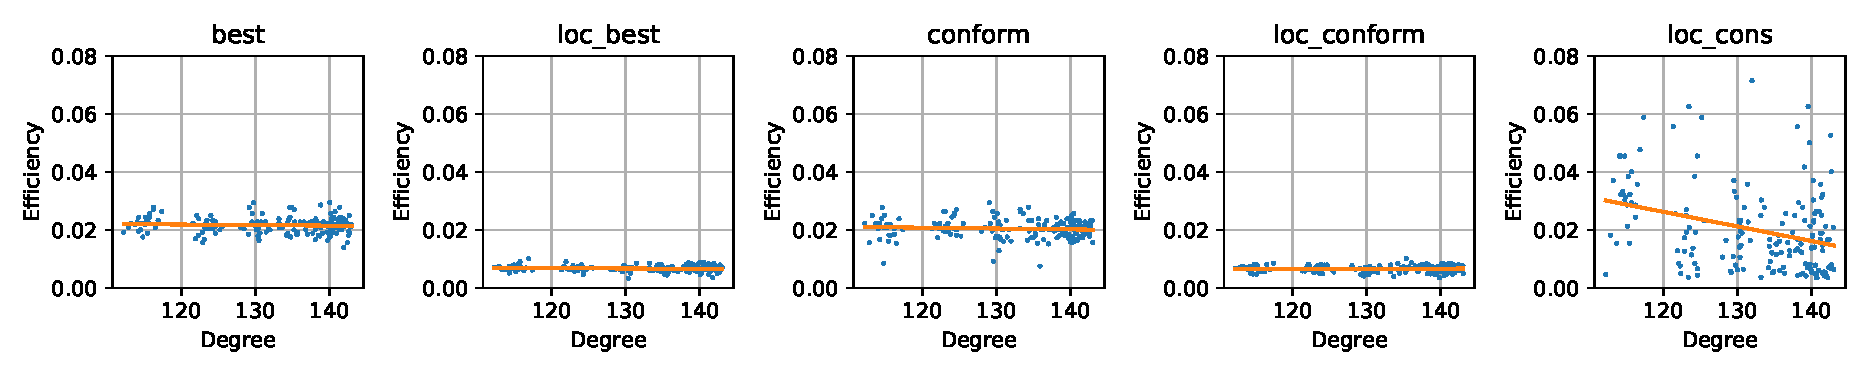
\includegraphics[width=6.67in,height=1.33in]{fig-deg-eff.pdf}
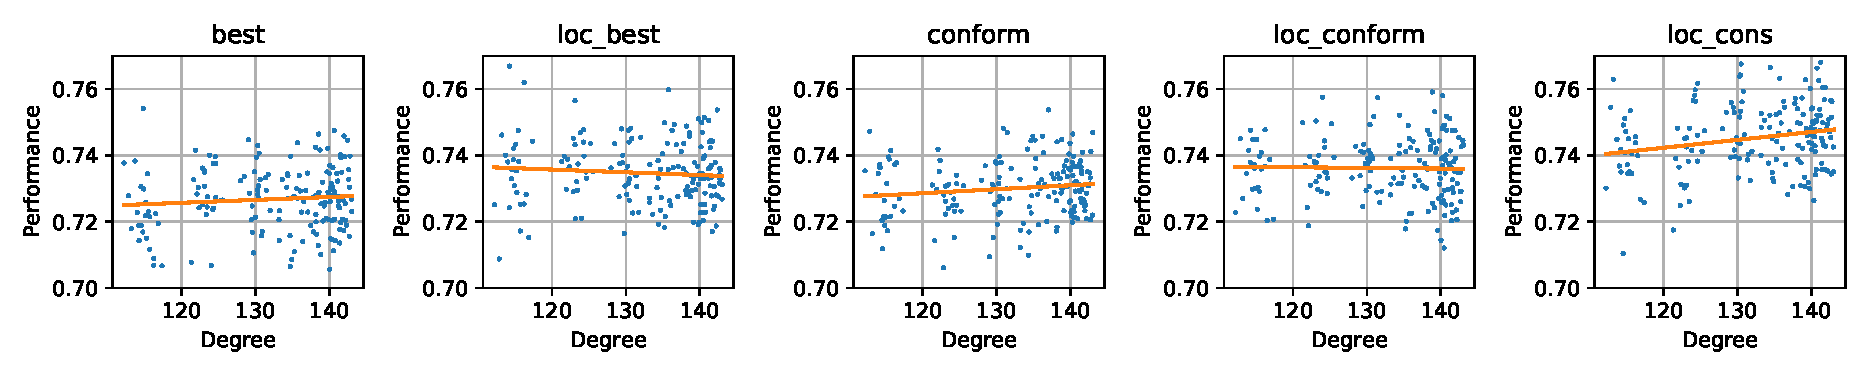
\includegraphics[width=6.67in,height=1.33in]{fig-deg-perf.pdf}
\caption{
Efficiency and Performance of social learning strategies vs network degree.
Each point represents a single trial of 300 iterations.
The consensus strategy shows increased performance and decreased efficiency as
degree increases, while other strategies show no degree dependence.
\label{fig:deg-eff-perf}
}
\end{figure*}

Figure \ref{fig:val-iter} shows how agents' solutions improve after repeated applications of
different learning strategies and rewiring values.
Each curve represents an average over 100 trials, each with 250 agent solutions.
For all rewiring values, local strategies are less efficient and more performant than their
non-local counterparts.
The consensus strategy is both more efficient and more performant than others,
with its performance increasing with higher rewiring.

The effect of degree on performance and efficiency is shown in Figure \ref{fig:deg-eff-perf} and
Tables \ref{tab:sim-eff} and \ref{tab:sim-perf}.
For both local and non-local versions of the best-neighbor and conformity strategies,
there is no significant effect of degree on performance or efficiency.
As noted above however, the local versions consistently have higher performance and lower efficiency
than their non-local counterparts.
We observe more interesting behavior with the consensus strategy.
Node degree shows a significant negative correlation with degree,
and a small but significant positive correlation with efficiency.
The consensus simulations replicate the efficiency behavior observed in WikiProjects,
but the opposite behavior for performance.
But unlike other strategies, consensus demonstrates that degree distribution can have an
impact on both performance and efficiency.

\section{Discussion}
\label{sec:discuss}

While existing research into the role of network structure in collaboration
has focused on numerical simulations and lab experiments,
analysis of large real-world systems is an important next step.
Our empirical analysis of WikiProjects contributes several findings towards a better
understanding of large, decentralized, real-world collaboration.
We observe several results consistent with previous work:
a trade-off between performance and efficiency,
higher performance for shorter path lengths in a conformity setting,
and a reduction in performance with increased structural inequality.
By using real-world networks, we were also able to analyze network properties independently,
allowing us to show that while most existing work has focused on the importance of path length,
degree distribution may be just as, or more, important.
The association of low-degree with both high performance and high efficiency is compelling,
as it sidesteps the usual trade-off between performance and efficiency.
In low-degree networks, agents have more repeated interactions with smaller groups of collaborators,
possibly suggesting that small team sizes could be beneficial for large collaborations.
Similarly, the observation that performance is higher in projects with less structural inequality suggests that,
if the challenges of egalitarian organizing can be overcome,
decentralized collaborations may produce better outcomes than those with centralized, top-down structures.

Our numerical simulations offer a few additional insights.
Our proposed local variants of best-neighbor and conformity strategies out-performed
the standard variants while searching fewer alternatives.
The higher performance for less work is analogous to the performance increases that
have been seen for sampling fewer neighbors \cite{barkoczi_social_2016}.
However, our network is a special case in that its structure is related to the structure of
the NK model being optimized, which could increase the usefulness of local information.
Our proposed consensus strategy, intended to model Wikipedia more closely,
exhibits a degree-dependent performance and efficiency, unlike other strategies.
This dependence is also seen in our Wikipedia analysis, although performance's dependence has the opposite sign.
The consensus strategy is also interesting in that it is more efficient and higher performance than the other strategies.
The unique properties of the consensus strategy may be due to a major difference it has from the others:
rather than exploring through local hill-climbing,
the consensus strategy combines parts of existing solutions to create entirely new ones.

Our work has several limitations.
Our empirical analysis is purely correlative and cannot be used to draw
conclusions about the causal influence of network structure on collaboration.
However, the consistency of our results with other lab-based and numerical studies
suggests that the causal link is worth further study.
Similarly, our study focuses entirely on a single setting and while it is suggestive,
does not necessarily generalize,
and studies of other systems are necessary to corroborate our findings.

Our work raises several questions that could be the subject of future work.
Is the correlation between network structure, performance, and efficiency causal?
A time-dependent analysis of our data could offer insight.
Are similar relationships observed in other large-scale collaborations?
Does varying degree independently of path length influence performance and efficiency in a controlled
lab setting?

\section{Conclusion}
\label{sec:conclusion}

In this paper, we have described the relationship between the structural properties of WikiProject
coeditor networks and the performance and efficiency of those networks.
As in other studies, we see a trade-off between performance and efficiency,
but not an absolute trade-off.
Some properties, such as low degree, are associated with both higher performance and higher efficiency.
We also find that the correlations between path length and performance are consistent with a conformity-based
social learning strategy, but not a greedy best-neighbor strategy.
We also observe improved performance in more decentralized project, as has been seen in small-scale lab experiments.
While the performance and efficiency of most previously-studied social learning strategies depend more on path length than
degree,
we have proposed a novel consensus learning strategy that is more realistic, more efficient, and higher performance than
existing strategies.
While the efficiency and performance of existing strategies do not exhibit any degree-dependence, our consensus strategy
demonstrates that degree-dependence is possible.
While additional work is needed to determine causal relationships and how generalizable our results are,
we have shown evidence that several phenomena predicted by numerical and small-scale lab experiments are present in a large,
real-world network.
And, we have identified new behaviors not explained by existing models, suggesting the need for alternate models.
Our results suggest that the success of large-scale collaborations may be aided by greater decentralization,
consensus or conformity-based decision-making, and more tightly-knit collaborations between smaller teams.

\section{Acknowledgments}
I would like to thank Daniel M. Romero for valuable guidance and feedback;
Ceren Budak and Scott E. Page for their time and feedback;
Danielle Livneh and Karthik Ramanathan for help collecting the data sets;
Yan Chen and Tanya Rosenblat for feedback on the methodology;
and the attendees of the May 25, 2017 MIT Center for Civic Media lab meeting and
the Berkman-Klein Center's Cooperation Working Group for helpful feedback on
preliminary results.
This research was funded by the University of Michigan School of Information.

% ACM
%\bibliographystyle{ACM-Reference-Format}

% Manuscript
\bibliographystyle{acm}

\bibliography{paper} 

\end{document}
